\documentclass{article}

\usepackage{amsmath}
\usepackage{amsfonts} % For math fonts.
\usepackage{amssymb} % For other math symbols not covered by amsmath.
\usepackage[pdftex]{graphicx} % For pictures, use %\includegraphics[scale=decimal]{pic.png}; must be a .png file type.
\usepackage{multicol}
\usepackage{textcomp}
\usepackage[colorlinks = true, urlcolor = blue]{hyperref}
\usepackage{enumitem}
\usepackage{graphbox} 
\usepackage{subfig}
\usepackage{multicol}

\newcommand{\tab}{\hspace*{0.25in}}

\usepackage{tikz}
\usetikzlibrary{positioning, calc}
\usetikzlibrary{shapes.geometric,angles,quotes}
\usepackage{tikz-3dplot}

\newcommand{\csq}[1]{\reflectbox{''}#1''}  %This produces CS style quotes.
\newcommand{\csqt}[1]{\text{\reflectbox{''}#1''}}  %This produces CS style quotes as text.



\usepackage{fullpage}
\usepackage{listings}
\lstset
{ %Formatting for code in appendix
    language=Python,
    basicstyle=\footnotesize,
    numbers=left,
    stepnumber=1,
    showstringspaces=false,
    tabsize=2,
    breaklines=true,
    breakatwhitespace=false,
}


\begin{document}


\begin{flushright}
classes 3\end{flushright}

\vspace*{-1.5em}
\noindent\makebox[\linewidth]{\rule{\paperwidth}{0.4pt}}


\vspace*{2em}

\begin{enumerate}

%standard 13.1


%start_of_questions

%new_question
%%%%%%%%%%%%%%%%%%%%%
	% Problem 1
	% Difficulty: 1
%%%%%%%%%%%%%%%%%%%%%
	\item
		Write a class for a \textbf{Vector} with the instance variables and methods listed below.\\
		A vector in the $xy$-plane is a quantity that has both direction and magnitude.\\ It can 
		be written in the form $v = ax + by$, where $a$ and $b$ are real numbers.\\[0.5em]
		Some examples of vectors include:
		
		\begin{minipage}[t]{0.65\textwidth}
			\begin{itemize}
				\item $v_1 = 3x + 2y$
				\item $v_2 = -2x + 6y$
				\item $v_3 = 2x$ (which is the same as $2x + 0y$)
			\end{itemize}

			Your class should support:
			\begin{itemize}
				\item Creating a vector with $x$ and $y$ components
				\item Comparing if two vectors are equal using the \_\_eq\_\_ method
				\item Printing a readable version of the vector
			\end{itemize}
		\end{minipage}
		\hfill
		\begin{minipage}[t]{0.32\textwidth}
			\vspace{-1.2em} % Adjust this value to align vertically with the sentence above
			\begin{flushright}
				\begin{tabular}{|l|}
					\hline
					Vector \\ \hline
					a (x-component) \\
					b (y-component) \\ \hline
					\_\_init\_\_ \\
					%\_\_add\_\_ \\
					\_\_eq\_\_ \\
					\_\_str\_\_ \\ \hline
				\end{tabular}
			\end{flushright}
		\end{minipage}
		
		Hint: Two vectors are equal if their components are equal. That is, the x-components 
		of both are equal and the y-components of both are equal.\\
		For example, $v_1 =(2x + 3y)$ and $v_2=(2x + 3y)$ are equal, \\
		but $v_1=(2x + 3y)$ and $v_2=(4x + 5y)$ are not.\\[0.5em]
		After writing the class, initialize three vectors and write code to add them together.

		%Hint: Vectors are added component-wise.\\
		%For example, $(2x + 3y) + (4x + 5y) = 6x + 8y$.\\[0.5em]
		%After writing the class, initialize three vectors and write code to add them together.




%new_question
%%%%%%%%%%%%%%%%%%%%%
	% Problem 2
	% Difficulty: 1
%%%%%%%%%%%%%%%%%%%%%
	\item
		Write a class for a \textbf{Point} with the instance variables and methods listed below.\\
		A point in the coordinate plane has an $x$ and $y$ coordinate. Points can be compared, 
		and the distance between two points can be calculated using the distance formula.
			
		\begin{minipage}[t]{0.65\textwidth}
			For example:
			\begin{itemize}
				\item $p_1 = (3, 4)$
				\item $p_2 = (0, 0)$
				\item Distance between $p_1$ and $p_2$ is $\sqrt{(3 - 0)^2 + (4 - 0)^2} = 5$
				%\item $p_1 + p_2 = (3 + 0,\ 4 + 0) = (3,\ 4)$
				\item $(3,4)$ is equal to $(3,4)$, but $(1,2)$ is not equal to $(6,6)$.
			\end{itemize}
		\end{minipage}
		\hfill
		\begin{minipage}[t]{0.32\textwidth}
			\vspace{.2em}
			\begin{flushright}
				\begin{tabular}{|l|}
					\hline
					Point \\ \hline
					x (x-coordinate) \\
					y (y-coordinate) \\ \hline
					\_\_init\_\_ \\
					\_\_eq\_\_ \\
					distance(other) \\
					\_\_str\_\_ \\ \hline
				\end{tabular}
			\end{flushright}
		\end{minipage}
		
		Your class should support:
		\begin{itemize}
			\item Creating a point with $x$ and $y$ coordinates
			%\item Adding two points using the \_\_add\_\_ method
			\item Determine if two points are equal using the \_\_eq\_\_  method	
			\item Calculating the distance to another point using \texttt{distance(other)}
			\item Printing a readable version of the point
		\end{itemize}
		
		Once you have created the class, add code that:
		\begin{itemize}
			\item Instantiate two Points
			\item Compare if they are equal
			\item Print a readable version of one of the Points you created.
			%\item Handles invalid input (e.g., wrong types or missing values)
		\end{itemize}




%new_question
%%%%%%%%%%%%%%%%%%%%%
	% Problem 7
	% Difficulty: 1
%%%%%%%%%%%%%%%%%%%%%
	\item
		Write a class for a \textbf{ComplexNumber} with the instance variables and methods listed 
		below.\\
		A ComplexNumber is a number of the form $a + bi$, where $a$ is the real part, $b$ is 
		the imaginary part, and both $a$ and $b$ are real numbers. 
			
		\begin{minipage}[t]{0.7\textwidth}
			Some examples of a ComplexNumber include:
			\begin{itemize}
				\item $z_1 = 3 + 2i$
				\item $z_2 = -1 + 4i$
				\item $z_3 = 2$ (which is the same as $2 + 0i$)
			\end{itemize}
		\end{minipage}
		\hfill
		\begin{minipage}[t]{0.25\textwidth}
			\vspace{.2em}
			\begin{flushright}
				\begin{tabular}{|l|}
					\hline
					ComplexNumber \\ \hline
					a (real part) \\
					b (imaginary part) \\ \hline
					\_\_init\_\_ \\
					\_\_eq\_\_ \\
					\_\_str\_\_ \\ \hline
				\end{tabular}
			\end{flushright}
		\end{minipage}
		
		Once you have created the class, add code that:
		\begin{itemize}
			\item Instantiates two ComplexNumbers with a real and imaginary parts
			%\item Adds two ComplexNumbers using the \_\_add\_\_ method
			\item Compares if two ComplexNumbers are equal using the \_\_eq\_\_  method		
			\item Printing a readable version (e.g., \csq{3 + 2$i$} or \csq{5 - 1$i$})
		\end{itemize}
		
		%Hint: ComplexNumbers are added component-wise.\\
		%For example, $(2 + 3i) + (4 + 5i) = 6 + 8i$.\\
		
		After writing the class, initialize two ComplexNumbers and write code to determine if
		they are equal.

%end_of_questions
%make sure to leave at least one blank line below



%standard 13.2


%start_of_questions



%new_question
%%%%%%%%%%%%%%%%%%%%%
	% Problem 3
	% Difficulty: 2
%%%%%%%%%%%%%%%%%%%%%
	\item
		Write a class for a \textbf{LinearEquation} with the instance variables and methods listed 
		below.\\ A linear equation is of the form $y = mx + b$, where $m$ is the slope and $b$ is 
		the $y$-intercept.

		\begin{minipage}[t]{0.65\textwidth}
				For example:
			\begin{itemize}
				\item $y_1 = 2x + 3$
				\item $y_2 = -x + 5$
			\end{itemize}
			You should be able to add two equations together:
			\begin{itemize}
				\item $y_1 + y_2 = (2 - 1)x + (3 + 5) = x + 8$
			\end{itemize}
		\end{minipage}
		\hfill
		\begin{minipage}[t]{0.32\textwidth}
			\vspace{0.2em}
			\begin{flushright}
				\begin{tabular}{|l|}
					\hline
					LinearEquation \\ \hline
					m (slope) \\
					b (y-intercept) \\ \hline
					\_\_init\_\_ \\
					%evaluate(x) \\
					\_\_add\_\_ \\
					\_\_str\_\_ \\ \hline
				\end{tabular}
			\end{flushright}
		\end{minipage}
		
		Your class should support:
		\begin{itemize}
			\item Creating a linear equation with slope and y-intercept
			%\item Evaluating the equation at a given $x$ using the \texttt{evaluate(x)} method
			\item Adding two equations using the \_\_add\_\_ method
			\item Printing a readable version of the equation
		\end{itemize}
		
		Once you have created the class, add code that:
		\begin{itemize}
			\item Instantiate two linear equations
			%\item Evaluates one at a specific $x$ value
			\item Add them together
			%\item Handles invalid inputs (e.g., non-numeric $x$ in evaluate)
			\item print a readable version of one of the LinearEquations you created.
		\end{itemize}



%new_question
%%%%%%%%%%%%%%%%%%%%%
	% Problem 4
	% Difficulty: 2
%%%%%%%%%%%%%%%%%%%%%
	\item
		Write a class for a \textbf{Time} object with the instance variables and methods listed 
		below.\\
		Time can be represented in hours and minutes (e.g., 2 hours and 45 minutes). \\
		When adding times, make sure minutes are correctly carried into hours.

		\begin{minipage}[t]{0.65\textwidth}
			For example:
			\begin{itemize}
				\item $t_1 = 1$ hour $30$ minutes
				\item $t_2 = 2$ hours $45$ minutes
				\item $t_1 + t_2 = 4$ hours $15$ minutes 
					(because $30 + 45 = 75$ minutes, which becomes $1$ hour $15$ minutes)
			\end{itemize}

		\end{minipage}
		\hfill
		\begin{minipage}[t]{0.32\textwidth}
			\vspace{.2em}
			\begin{flushright}
				\begin{tabular}{|l|}
					\hline
					Time \\ \hline
					hours \\
					minutes \\ \hline
					\_\_init\_\_ \\
					\_\_add\_\_ \\
					\_\_str\_\_ \\ \hline
					%to\_minutes \\ 
				\end{tabular}
			\end{flushright}
		\end{minipage}
		
		Your class should support:
		\begin{itemize}
			\item Creating a time object with hours and minutes
			\item Adding two times using the \_\_add\_\_ method 
				%(properly handling minutes overflow)
			\item Printing time in a readable format (e.g., \csq{2h 45m})\\
				Hint: you don't need to consider days. You can have 30 hours.
			%\item Converting total time to just minutes using \texttt{to\_minutes()}
		\end{itemize}

		Once you have created the class, add code that:
		\begin{itemize}
			\item Creates two time objects
			\item Adds them together
			\item Prints the result
			%\item Shows the total number of minutes
			%\item Includes error handling for negative values or invalid types
		\end{itemize}



%new_question
%%%%%%%%%%%%%%%%%%%%%
	% Problem 5
	% Difficulty: 2
%%%%%%%%%%%%%%%%%%%%%
	\item
		Write a class for an \textbf{RGBColor} with the instance variables and methods listed 
		below. Colors on a screen are often represented using Red, Green, and Blue components 
		(values from 0 to 255).\\
		Colors can be added together by taking the average of adding each component.

		\begin{minipage}[t]{0.7\textwidth}
			Some examples of RGB colors:
			\begin{itemize}
				\item $c_1 = (170,\ 150,\ 200)$
				\item $c_2 = (30,\ 100,\ 60)$
				\item $c_3 = c_1 + c_2 = (\frac{170+30}{2},\ \frac{150+100}{2},\ \frac{200+60}{2})$ 
					becomes $(100,\ 125,\ 130)$
			\end{itemize}
		
			Your class should support:
			\begin{itemize}
				\item Creating a color with red, green, and blue values (each from 0 to 255)
				\item Adding two colors using the \_\_add\_\_ method (cap each result at 255)
				\item Printing the color in a readable format (e.g.,\csq{RGB(150, 200, 255)})
			\end{itemize}
		\end{minipage}
		\hfill
		\begin{minipage}[t]{0.25\textwidth}
			\vspace{.2em}
			\begin{flushright}
				\begin{tabular}{|l|}
					\hline
					RGBColor \\ \hline
					r (red) \\
					g (green) \\
					b (blue) \\ \hline
					\_\_init\_\_ \\
					\_\_add\_\_ \\
					\_\_str\_\_ \\ \hline
				\end{tabular}
			\end{flushright}
		\end{minipage}
		
		After writing the class, create three colors and write code to add them together.
		Print the result.

	

%new_question
%%%%%%%%%%%%%%%%%%%%%
	% Problem 6
	% Difficulty: 2
%%%%%%%%%%%%%%%%%%%%%
	\item
		Write a class for a \textbf{RationalNumber} with the instance variables and methods 
		listed below.\\
		A RationalNumber is a number that can be expressed as the ratio of two integers: 
		$\dfrac{a}{b}$, where $b \ne 0$.

		\begin{minipage}[t]{0.65\textwidth}
			Some examples of RationalNumber addition include:
			\begin{itemize}
				\item $\dfrac{1}{3} + \dfrac{1}{2} = \dfrac{5}{6}$ (not $0.8333\ldots$)
				\item $\dfrac{2}{5} + \dfrac{1}{5} = \dfrac{3}{5}$
			\end{itemize}
		\end{minipage}
		\hfill
		\begin{minipage}[t]{0.32\textwidth}
			\vspace{.2em}
			\begin{flushright}
				\begin{tabular}{|l|}
				\hline
				RationalNumber \\ \hline
				numerator \\
				denominator \\ \hline
				\_\_init\_\_ \\
				\_\_add\_\_ \\
				\_\_str\_\_ \\ \hline
				\end{tabular}
			\end{flushright}
		\end{minipage}
		
		Your class should support:
		\begin{itemize}
			\item Creating a rational number with a numerator and denominator
			\item Adding two rational numbers using the \_\_add\_\_ method 
			\item Printing a readable version (e.g., as a fraction)
		\end{itemize}
		
		Hint: To add fractions, find a common denominator.\\
		For example, $\dfrac{1}{3} + \dfrac{1}{2} = \dfrac{2}{6} + \dfrac{3}{6} = \dfrac{5}{6}$.\\
		\newline
		After writing the class, create two rational numbers and demonstrate adding and printing.




%new_question
%%%%%%%%%%%%%%%%%%%%%
	% Problem 10
	% Difficulty: 2
%%%%%%%%%%%%%%%%%%%%%
	\item
		Write a class for a \textbf{Rectangle} with the instance variables and methods 
		listed below.\\
		A Rectangle has a width and a height. You should be able to calculate its area	and multiply 
		a Rectangle by an integer. The result of multiplying by an integer should be that the height 
		and width of the current Rectangle are multiplied (modified) by the integer value.
		%When a rectangle is multiplied by an integer the result should be that the current 
		%rectangle has both its height and width modified by that integer value. 

		\begin{minipage}[t]{0.7\textwidth}
			Some examples:
			\begin{itemize}
				\item $r_1 = \text{width: } 4,\ \text{height: } 5$
				\item $r_2 = \text{width: } 3,\ \text{height: } 2$
				\item $r_1 * 3 = \text{width: } 12,\ \text{height: } 15$
			\end{itemize}

			\begin{minipage}{0.25\textwidth}
				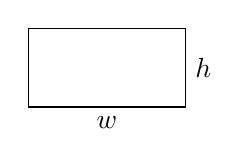
\begin{tikzpicture}
					\draw (0,0)  -| (2,1) 
						node[pos=0.25,below] {$w$} 
						node[pos=0.75,right] {$h$}
						-| (0,0);
				\end{tikzpicture}
			\end{minipage}
			{\Large $\longrightarrow$} \hspace*{2em}
			\begin{minipage}{0.65\textwidth}
				\begin{tikzpicture}
					\draw (0,0)  -| (6,3) 
						node[pos=0.25,below] {$3 \cdot w$} 
						node[pos=0.75,right] {$3 \cdot h$}
						-| (0,0);
				\end{tikzpicture}
			\end{minipage}
		\end{minipage}
		\hfill
		\begin{minipage}[t]{0.2\textwidth}
			\vspace{.2em}
			\begin{flushright}
				\begin{tabular}{|l|}
					\hline
					Rectangle \\ \hline
					width \\
					height \\ \hline
					\_\_init\_\_ \\
					area() \\
					%perimeter() \\
					\_\_mul\_\_ \\
					\_\_str\_\_ \\ \hline
				\end{tabular}
			\end{flushright}
		\end{minipage}
		
		Your class should support:
		\begin{itemize}
			\item Creating a rectangle with width and height.
			\item Calculating the area using \texttt{area()}.
				%and perimeter using \texttt{perimeter()}
			\item Multipying a rectangle by an integer using the  \_\_mul\_\_ method.
			\item Printing the rectangle in a readable format (e.g., \csq{Rectangle(4 x 5)})
		\end{itemize}
		
		Once you have created the class, add code that:
		\begin{itemize}
			\item Creates a rectangle
			\item Multiplies it by an integer.
			\item Prints the result
		\end{itemize}

%end_of_questions
%make sure to leave at least one blank line below


%standard 13.3



%start_of_questions


%new_question
%%%%%%%%%%%%%%%%%%%%%
	% Problem 8
	% Difficulty: 3
%%%%%%%%%%%%%%%%%%%%%
	\item % give playlist default name.
		Write a class for a \textbf{Playlist} with the instance variables and methods listed 
		below.\\
		A Playlist should have a default name of \csq{New Playlist}.\\
		It can be instantiated with initial songs, but it is not required to.\\
		Create a method called \textit{add\_song} which adds a song title (a string) to the 
		Playlist.\\
		You should be able to combine two Playlists, and print them in a readable way.
			
		\begin{minipage}[t]{0.65\textwidth}
			For example:
			\begin{itemize}
				\item $p_1 = [\csqt{Song A}, \csqt{Song B}]$
				\item $p_2 = [\csqt{Song C}]$
				\item $p_1 + p_2 = [\csqt{Song A}, \csqt{Song B}, \csqt{Song C}]$
			\end{itemize}

			Your class should support:
			\begin{itemize}
				\item Creating a playlist with a name and list of songs
				\item Adding two playlists (combines song lists)
				\item Printing the playlist in a readable way (e.g., list songs)
			\end{itemize}	
		\end{minipage}
		\hfill
		\begin{minipage}[t]{0.32\textwidth}
			\vspace{.2em}
			\begin{flushright}
				\begin{tabular}{|l|}
					\hline
					Playlist \\ \hline
					name \\
					songs (list of strings) \\ \hline
					\_\_init\_\_ \\
					add\_song \\
					\_\_add\_\_ \\
					\_\_str\_\_ \\ \hline
				\end{tabular}
			\end{flushright}
		\end{minipage}
		
		Once you have created the class, add code that:
		\begin{itemize}
			\item Creates two playlists and at least one song to each.
			\item Combines the playlists
			\item Prints the result
		\end{itemize}



%new_question
%%%%%%%%%%%%%%%%%%%%%
	% Problem 9
	% Difficulty: 3
%%%%%%%%%%%%%%%%%%%%%
	\item
		Write a class for a \textbf{ShoppingCart} with the instance variables and methods listed 
		below.\\
		It can be instantiated with initial items in the cart, but it is not required to.\\
		Create a method called \textit{add\_items} which adds an item (a string) to the 
		ShoppingCart. The same item can be added more than once. If the item is already in the 
		ShoppingCart, increase its quantity by one. If its not in the ShoppingCart, set the 
		quantity to 1.\\ Hint: think about what type of data structure you should use. \\
		When two ShoppingCarts are added together, the result should be a ShoppingCart 
		containing the items in both. Overlapping items should have a sum of their quantities.

		\begin{minipage}[t]{0.65\textwidth}
			For example:
			\begin{itemize}
				\item $p_1 = \{\csqt{tea}:1, \csqt{energy drink}:2 \}$
				\item $p_2 = \{\csqt{energy drink}:3, \csqt{hat}:1 \}$
				\item $p_1 + p_2 = \{\csqt{tea}:1, \csqt{energy drink}:5, \csqt{hat}:1 \}$
			\end{itemize}		
		\end{minipage}
		\hfill
		\begin{minipage}[t]{0.32\textwidth}
			\vspace{0.1em}
			\begin{flushright}
				\begin{tabular}{|l|} \hline
					ShoppingCart \\ \hline
					items (dict$\rightarrow$str:int) \\ \hline
					\_\_init\_\_ \\
					add\_item \\
					\_\_add\_\_ \\
					\_\_str\_\_ \\ \hline
				\end{tabular}
			\end{flushright}
		\end{minipage}
		
		Your class should support:
		\begin{itemize}
			\item Creating a ShoppingCart
			\item Adding two ShoppingCarts (combines items)
			\item Printing the ShoppingCart in a readable way 
				(e.g., lists all items with quantities)
		\end{itemize}
		
		Once you have created the class, add code that:
		\begin{itemize}
			\item Creates two ShoppingCarts and at least one item to each.
			\item Combines the ShoppingCarts
			\item Prints the result
		\end{itemize}

%end_of_questions
%make sure to leave at least one blank line below



\end{enumerate}
\end{document}

